Minęło ponad 70 lat odkąd Warren McCulloch i Walter Pitts stworzyli pierwszą sztuczną sieć neuronową (\acrshort{ann}), która odwzorowywała sposób pracy mózgu \cite{dnn_first}. Sukcesywnie \acrshort{ann} zyskiwały na popularności i ostatecznie stały się jednym z najpotężniejszych narzędzi uczenia maszynowego, a ich skuteczność została przetestowana w wielu dziedzinach nauki. W połączeniu z głębokim uczeniem sztuczne sieci neuronowe odniosły niewątpliwy sukces. Podsumowanie najważniejszych osiągnięć \acrshort{dnn} można znaleźć w obszernej pracy \cite{dnn_overview}. Ponadto \acrshort{dnn} mają szczególne zasługi w przetwarzaniu języka naturalnego (opracowania języka angielskiego), przewyższając niejednokrotnie zdolności percepcyjne człowieka \cite{ds2, ds3_top1, ds3_top2}. Liczna grupa naukowców pracowała na sukces sztucznych sieci neuronowych w tym polscy przedstawiciele m.in prof. Ryszard S. Michalski. 

Ten rozdział odnosi się do niezbędnej teorii, aby móc zrozumieć podstawowe modele rozpoznawania mowy w pełni oparte na głębokim uczeniu. 

\section{Artifical Neuron}
Koncepcja \acrshort{ann} została zainspirowana naturą. Ludzki mózg składa się z połączonych komórek zwanymi neuronami, które przekazują wzajemnie informację za pomocą sygnałów elektrycznych i chemicznych. Połączenia między neuronami są nazywane \textit{aksonami}. Jeśli suma sygnału przychodzącego jest wystarczająca do \textit{aktywacji} neuronu, przekaże on rezultat pracy swojej komórki poprzez \textit{akson} do wszystkich przyłączonych z nim neuronów. Ludzki mózg zawiera około $10^{11}$ neuronów, z których każdy łączy średnio 10 tyś. innych. Najszybszy czas przejścia sygnału przez neuron wynosi $10^{-3}$ sekundy, czyli znacznie wolniej niż komputer ($10^{-10}$ sekundy) \cite{ml_book}. Mimo wszystko ludzki umysł korzysta z sieci neuronów w zaskakująco efektywny sposób i z łatwością rozwiązuje złożone problemy tj. rozpoznawanie mowy. 
\begin{figure}[ht]
    \centering
    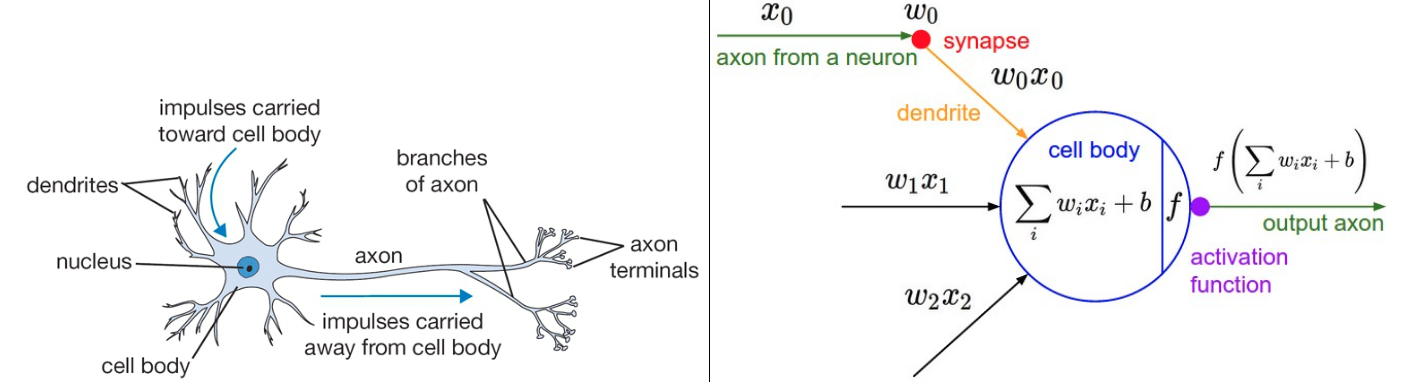
\includegraphics[width=0.8\textwidth]{images/neuron_and_perceptron.png}
    \caption{Schemat neuronu oraz jego matematyczna reprezentacja: \textit{perceptron} \cite{cs231n}}
    \label{fig:perceptron}
\end{figure}

Sztuczne sieci neuronowe (\acrshort{ann}) odzwierciedlają biologiczny układ nerwowy. Podstawową jednostką sieci jest \emph{perceptron} (\ref{fig:perceptron}). Perceptron zbiera informacje ze środowiska lub innych perceptronów. Następnie przypisuje każdemu wejściu wagę synaptyczną (analogia do synaps), co prowadzi do ustalenia znaczenia poszczególnych sygnałów. Perceptron sumuje wszystkie sygnały wejściowe, dodaje swoją stałą (wyraz wolny funkcji liniowej) i przekształca sygnał zgodnie ze swoją funkcją \emph{aktywacji}. Niech $x$ będzie wektorem wejściowym, $w$ odpowiednimi wagami synaptycznymi, $b$ wyrazem wolnym (\emph{bias}) oraz $\varphi$ funkcją aktywacji. Wartością zwracaną przez perceptron jest:
\begin{equation} \label{eq:perceptron}
y=\varphi(w \cdot x + b) 
\end{equation}

Wizualną reprezentacją działania perceptronu jest hiperpłaszczyzna w przestrzeni $n$-wymiarowej, gdzie $n$ to liczba wymiarów danych wejściowych. Funkcja aktywacji jest kluczowym elementem perceptronu. Przekształcenie przestrzeni bez funkcji aktywacji jest liniowe, dlatego długi szereg połączonych ze sobą perceptronów może być zredukowany do jednego perceptronu (\textit{affine transformation}). Funkcje aktywacji są nieliniowe, a najbardziej popularne przedstawiono na rys. \ref{fig:activation_fun}. Wybranie \emph{nieliniowości} zależy od zastosowania i nie jest ściśle określone. Obliczenie pochodnej funkcji nie może być złożone ze względu na algorytm trenowania (\textit{backpropagation}). Prowadzone są badania nad zmieniającymi się podczas treningu funkcjami aktywacji \cite{activation_func_train}. 

\begin{align*}
&sigmoid(x) =  \frac {1} {1 + e^{-x}} &tanh(x) = \frac {e^x - e^{-x}} {e^x + e^{-x}}\\
&softplus(x) = ln(1 + e^x) &ReLU(x) = max(0, x)
\end{align*}

\begin{figure}
    \centering
    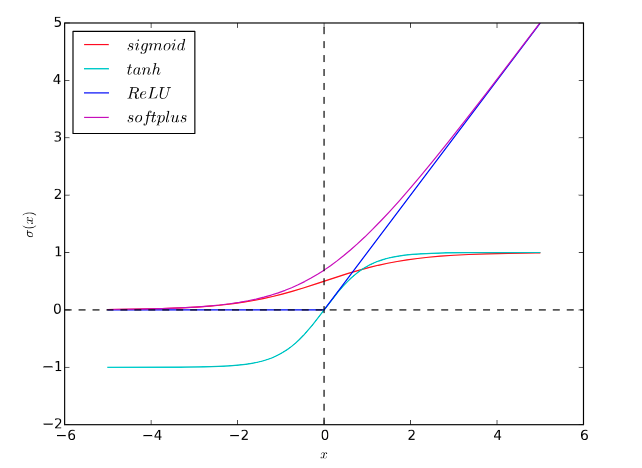
\includegraphics[width=0.6\textwidth]{images/activation_functions.png}
    \caption{Popularne funkcje aktywacji \cite{activation_func_train}}
    \label{fig:activation_fun}
\end{figure}

\section{Artifical Neural Network Architectures}
Pojedyncze perceptrony, inaczej jednostka (\textit{unit}), grupowane są w warstwę (\textit{layer}). Warstwa jest podstawowym elementem sieci. Istnieją trzy główne rodzaje warstw: \textit{fully connected}, \textit{recurrent} oraz \textit{convolutional}. Na ich podstawie zostały zbudowane podstawowe architektury: \acrfull{fnn},  \acrfull{rnn} oraz \acrfull{cnn}. Nowe kombinacje warstw tworzą nowe architektury.

\begin{figure}
    \centering
    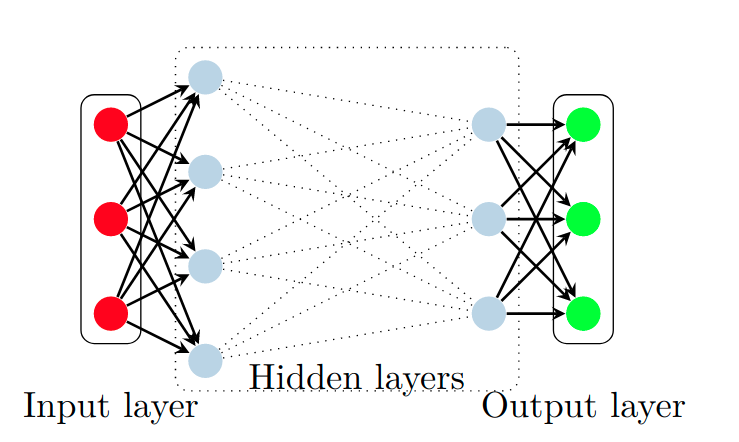
\includegraphics[width=0.5\textwidth]{images/arch_schema.png}
    \caption{Ogólny schemat sieci \acrshort{ann}}
    \label{fig:arch_schema}
\end{figure}

Wszystkie sieci \acrshort{ann} posiada warstwę: wejścia (\textit{input layer}) oraz wyjścia (\textit{output layer}) (rys. \ref{fig:arch_schema}). \textit{Input layer} wyłącznie wprowadza informacje, dlatego nie posiada perceptronów i nie jest wliczana do warstw modelu. Wszystkie wewnętrzne warstwy nazywamy \emph{ukrytymy} (\textit{hidden layer}). 

\subsection*{\acrfull{fnn}}
Podstawową architekturą sztucznych sieci neuronowych jest \acrshort{fnn} (inaczej \textit{multilayer perceptron}). Od lat 70 XX w. w \textit{tradycyjnych} rozwiązaniach rozpoznawania mowy sieć \acrshort{fnn} pełniła rolę transduktora, wyłącznie wspierając ukryte modele Markova \cite{ds1:feature_learning, ds1:dnn_timit, ds1:accustic_modeling, ds1:dnn_hmh}. 

Sieć \acrshort{fnn} złożona jest z warstw perceptronów w pełni połączonych (\acrshort{fc}). Każda jednostka (perceptron) w warstwie \acrshort{fc} jest połączona ze wszystkimi jednostkami w poprzedniej i następnej warstwie. Na rys. \ref{fig:feedforward_nn} przedstawiono przykład sieci \acrshort{fnn} złożonej z dwóch warstw. 

\begin{figure}
    \centering
    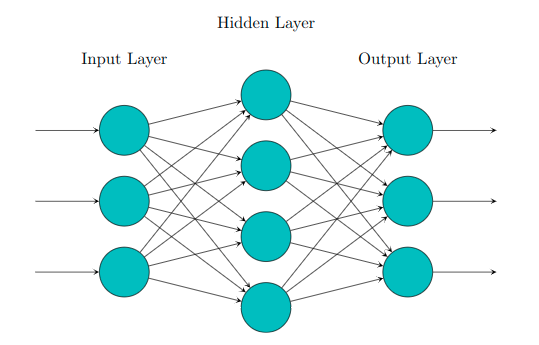
\includegraphics[width=0.5\textwidth]{images/feedforward_nn.png}
    \caption{Sieć \acrshort{fnn} z jedną warstwą ukrytą}
    \label{fig:feedforward_nn}
\end{figure}

Niech $l$ będzie numerem warstwy modelu $l=1...L$, gdzie $L$ to całkowita liczba warstw. Wartości zwracane przez warstwę $l$ modelu \acrshort{fnn} można opisać wzorem:
\begin{equation}
h^{(l)} = \varphi^{(l)} (\mathbb{W}^{(l)} \cdot h^{(l-1)} + b^{(l)})
\end{equation}
gdzie $h^{(l-1)}$ wartości wchodzące, $\mathbb{W}^{(l)}$ macierz wag synaptycznych, $b^{(l)}$ wyrazy wolne oraz funkcja aktywacji $\varphi^{(l)}$. Równanie jest rozszerzeniem opisu perceptronu (\ref{eq:perceptron}) do postaci macierzowej. 

\subsection*{\acrfull{rnn}}
Zastosowanie architektury \acrshort{rnn} w systemach rozpoznawania mowy było przełomowe. Analiza wąskiego fragmentu bez \emph{kontekstu} jest niemożliwa. Ludzki umysł podczas słuchania przetwarza całe sekwencje dźwięków. Warstwa \emph{rekurencyjna} w sieci \acrshort{rnn} tworzy kontekst poprzez zdolność utrzymania informacji w swojej strukturze.

\begin{figure}
    \centering
    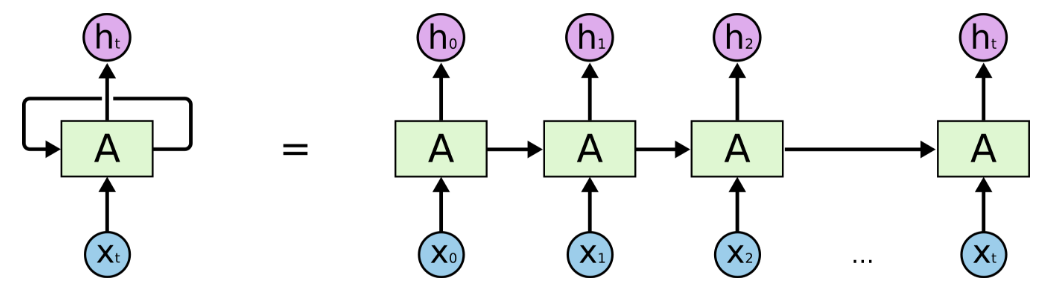
\includegraphics[width=0.7\textwidth]{images/rnn.png}
    \caption{Warstwa \acrshort{rnn} posiada pętle \cite{lstm:colah}}
    \label{fig:rnn}
\end{figure}

Warstwa rekurencyjna w odróżnieniu do \acrshort{fc} posiada \emph{pętle}, dzięki którym informacja jest przekazywana do następnego kroku (\ref{fig:rnn}). Pierwszą architekturę \acrshort{rnn} w latach 90 XX w. przedstawił J. Elman \cite{rnn}. Sieć jest złożona z dwóch warstw, a warstwa ukryta posiada pętle. 

\begin{figure}
    \centering
    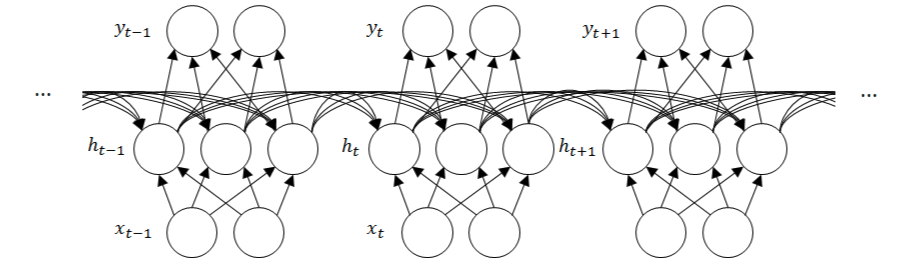
\includegraphics[width=0.7\textwidth]{images/rnn_concept.png}
    \caption{Pierwsza architektura \acrshort{rnn} \cite{rnn}}
    \label{fig:rnn-2}
\end{figure}

Warstwa rekurencyjna otrzymuje wąski fragment informacji $x_t$ oraz kontekst kroku poprzedniego $h_{t-1}$. Dodatkowa macierz wag $\mathbb{W}^{(h)}$ określa wpływ kontekstu na działanie komórki rekurencyjnej (\textit{recurrent cell}). Na podstawie sekwencji danych wejściowych $x_1, x_2, ..., x_T$, wartość zwracana przez sieć \acrshort{rnn} wynosi:

\begin{align}
&h_t = \varphi^{h} (\mathbb{W}^{(in)} \cdot x_t + \mathbb{W}^{(h)} \cdot h_{t-1} + b^{(in)})\\
&\hat{y} = \varphi^{o} (\mathbb{W}^{(out)} \cdot h_t +  b^{(out)})
\end{align}

\subsubsection*{\acrfull{lstm}}
Zaprezentowana prosta sieć \acrshort{rnn} interpretuje kontekst, dlatego m.in. w rozpoznawaniu mowy osiąga lepsze wyniki niż statyczne sieci \acrshort{fnn} \cite{rnn_over_fnn}. Teoretycznie \acrshort{rnn} jest w stanie, poprzez kontekst kroku poprzedniego i odpowiednio dobrane wagi $\mathbb{W}^{(h)}$, interpretować długie zależności (\textit{long-term dependencies}). Niestety metody trenowania modelu oparte na algorytmie gradientu prostego (\textit{gradient descent}) uniemożliwiają identyfikację długich zależności. Teoretyczne i eksperymentalne dowody zostały przedstawione w pracy \cite{rnn_long-term-problems}.

\begin{figure}
    \centering
    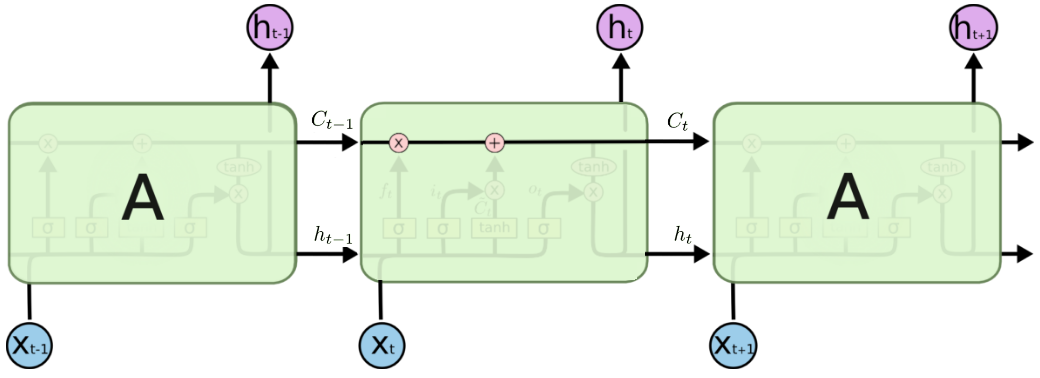
\includegraphics[width=0.8\textwidth]{images/lstm-1.png}
    \caption{Połączone komórki \acrshort{lstm} (zaadoptowane z \cite{lstm:colah})}
    \label{fig:lstm-1}
\end{figure}

Warstwa \acrfull{lstm} jest szczególnym rodzajem warstwy rekurencyjnej, która potrafi odkrywać długie zależności \cite{lstm}. Wszystkie sieci \acrshort{ann} na podstawie fragmentu danych $x_t$ starają się postawić trafną hipotezę $h_t$. Warstwy rekurencyjne posiadają dodatkowo pętle $h_{t-1}$, która pozwala analizować kontekst. Komórka \acrshort{lstm} dysponuje również informacją na temat stanu komórki z poprzedniego kroku $C_{t-1}$ (\textit{cell state}). Stan komórki $C$ to wektor opisujący \emph{ogólny} kontekst. Zmiany stanu ograniczone do dwóch operacji (\textit{pointwise operations}) są spowolnione w stosunku do pętli $h_{t-1}$ (rys. \ref{fig:lstm-1}).

\begin{figure}
    \centering
    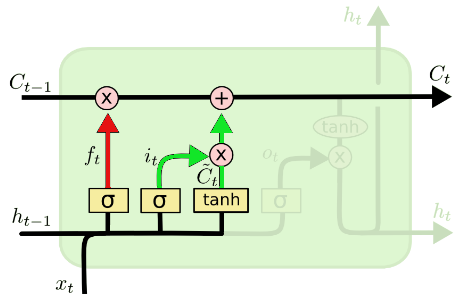
\includegraphics[width=0.5\textwidth]{images/lstm-2.png}
    \caption{Modyfikacja stanu komórki \acrshort{lstm} (zaadoptowane z \cite{lstm:colah})}
    \label{fig:lstm-2}
\end{figure}

Stan komórki jest modyfikowany za pomocą dwóch bram (\textit{gates}) na podstawie wektorów $h_{t-1}$ i $x_t$ (rys. \ref{fig:lstm-2}). \textit{Forget gate layer} (zaznaczona na czerwono) dzięki warstwie \textit{sigmoid} i \textit{pointwise multiplication} decyduje, które cechy odrzucić w ogólnym kontekście $C$. \textit{Input gate layer} (zaznaczona na zielono) określa, które cechy zostaną dodane. Warstwa $tanh$ tworzy grupę potencjalnych kandydatów nowych cech $\tilde{C_t}$. Wybrane cechy są dodane do stanu komórki. Aktualny kontekst $C_t$ jest wyznaczony (\ref{eq:lstm_state_update}). 
\begin{align}
&f_t = \sigma(\mathbb{W}^{(f)} \cdot [h_{t-1}, x_t] + b^{(f)}) \\
&i_t = \sigma(\mathbb{W}^{(i)} \cdot [h_{t-1}, x_t] + b^{(i)}) \\
&\tilde{C_t} = \tanh(\mathbb{W}^{(C)} \cdot [h_{t-1}, x_t] + b^{(C)}) \\
&C_t = f_t \circ C_{t-1} + t_t \circ \tilde{C_t} \label{eq:lstm_state_update}
\end{align}

Ostatnim etapem jest \textit{output gate layer}. \acrshort{lstm} zwraca hipotezę $h_t$ na podstawie stanu komórki $C_t$ z uwzględnieniem filtra $o_t$. 
\begin{align}
&o_t = \sigma(\mathbb{W}^{(o)} \cdot [h_{t-1}, x_t] + b^{(o)}) \\
&h_t = o_t \circ \tanh{C_t}
\end{align}

\begin{figure}
    \centering
    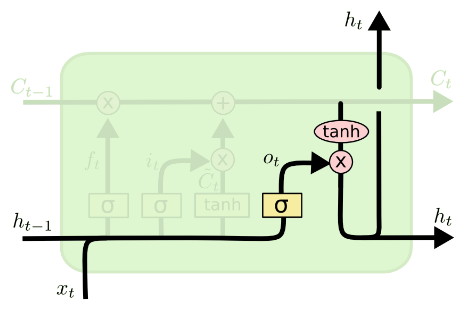
\includegraphics[width=0.5\textwidth]{images/lstm-3.png}
    \caption{Wartość zwracana komórki \acrshort{lstm} (zaadoptowane z \cite{lstm:colah})}
    \label{fig:lstm-3}
\end{figure}

% \subsection*{Bidirectional}
% \subsection*{Convolutional layer}

\section{Funkcja celu}
Wszystkie sieci neuronowe posiadają \emph{funkcję celu} $\mathcal{L}$ (\textit{objective/loss/cost function}), która ocenia skuteczność predykcji. W zależności od dziedziny problemu istnieje wiele różnych funkcji celu. Przykładowo niech problem dotyczy regresji liniowej. Model na podstawie kwoty na rachunku (dane wejściowe $X$) stara się przewidzieć wielkość napiwku (wzorcowe dane wyjściowe $Y$). Funkcją celu w takim przypadku może być średni błąd kwadratowy (\acrshort{mse} lub inaczej \acrshort{ols}). \acrshort{mse} opisuje średnią sumę kwadratów odległości każdego punktu obserwacji $y^{(i)}$ do estymowanej linii regresji $\hat{y}^{(i)}$ (\ref{eq:regression}).

\begin{equation}
\mathcal{L} = \frac{1}{n}\sum_{i=1}^n (y^{(i)} - \hat{y}^{(i))^2} \label{eq:regression}
\end{equation}

W dziedzinie rozpoznawania mowy sekwencja danych wejściowych $X=[x_1, x_2, ..., x_T]$ to najczęściej cechy stworzone na podstawie danych audio. Sekwencja $X$ jest mapowana na sekwencje transkrypcji $Y=[y_1, y_2, ..., y_U]$. Model zwraca hipotezę $\Hat{Y}$, która jest najbardziej prawdopodobna pod warunkiem wystąpienia $X$ (\textit{conditional probability}).

\begin{equation}
\Hat{Y} = \underset {Y}{\operatorname{argmax}} \ p(Y | X)
\end{equation}

Pozycje liter z transkrypcji nie są znane. Kolejne dane wejściowe $x_i$ nie muszą odpowiadać kolejnym literom z transkrypcji $y_i$, dlatego długości $X$ i $Y$ mogą być różne ($T >= U$). Słowa są wypowiadane w różnym tempie, więc stosunek długości $X$ i $Y$ może się zmieniać. Metody wyrównania fragmentów danych do liter są złożone i nieefektywne. Algorytm \acrshort{ctc} rozwiązuje ww. problemy.

\subsubsection*{\acrfull{ctc}}
Algorytm \acrshort{ctc} po raz pierwszy został przedstawiony w 2006 \cite{ctc}, a pierwsze eksperymenty na zbiorze \textit{TIMIT} (zbiór testowy rozpoznawania fonemów) zostały wykonane w 2011 \cite{ctc-first-imp}. Algorytm nie wymaga wyrównania pomiędzy $X$ i $Y$ (\textit{alignment-free}). 

\begin{figure}
    \centering
    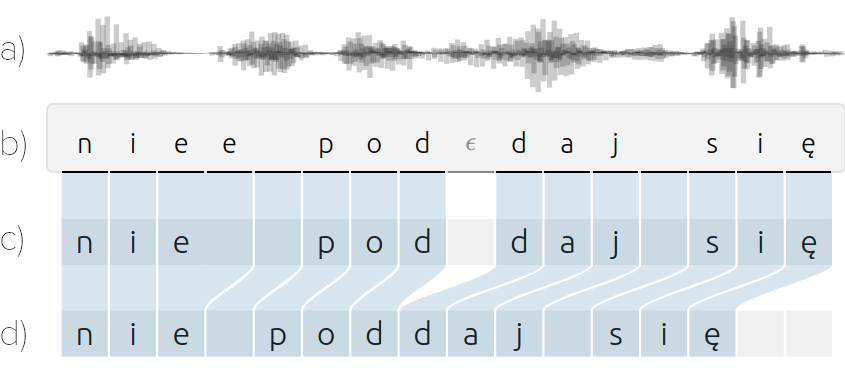
\includegraphics[width=0.5\textwidth]{images/ctc.png}
    \caption{Przykład wyrównania w algorytmie \acrshort{ctc} (zaadoptowane z \cite{ctc-distil})}
    \label{fig:ctc}
\end{figure}

Przykładowy model analizuje wyrażenie \say{nie poddaj się} (rys. \ref{fig:ctc}a). Na podstawie danych wejściowych $X$ w każdym kroku model zwraca \emph{wyłącznie} najbardziej prawdopodobną literę $a$ dostępną w alfabecie (rys. \ref{fig:ctc}b). Do alfabetu dodany jest dodatkowy pusty symbol $\epsilon$. Sekwencja wybranych liter tworzy wyrównanie $A$ (\textit{alignment}). Wyrównanie jest marginalizowane tzn. sekwencje powtarzających się liter są scalane w pojedyncze litery oraz puste tokeny $\epsilon$ zostają usunięte (rys. \ref{fig:ctc}c). Dzięki $\epsilon$ możliwa jest reprezentacja podwójnych liter oraz cisza w nagraniu dźwiękowym może zostać pominięta. Wyrównanie \acrshort{ctc} posiada właściwość \emph{wiele-do-jednego}. Może istnieć wiele wyrównań $A$, które po marginalizowaniu sprowadzają się do jednego wyniku (rys. \ref{fig:ctc}d). 

Model rozpoznawania mowy zwraca rozkład prawdopodobieństwa $p_t(a|X)$ \emph{wszystkich} dostępnych liter $a$ w alfabecie w kolejnych krokach $t$. Na podstawie prawdopodobieństw obliczane są wszystkie możliwe poprawne wyrównania $A$ (\textit{valid alignments}), które sprowadzają się do wyniku $Y$. Naiwne obliczenie wszystkich kombinacji $A$ jest nieefektywne, dlatego stosowany jest algorytm dynamicznego programowania. Kluczem jest scalanie tożsamych częściowych wyrównań $Z_{1:s}$ występujących w tym samym czasie $t$.  

\begin{figure}
    \centering
    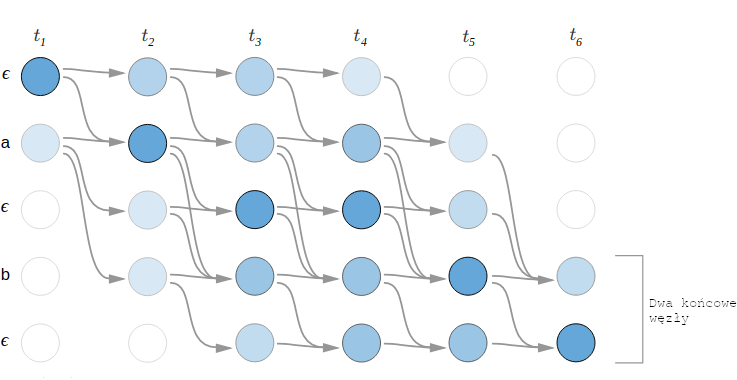
\includegraphics[width=0.7\textwidth]{images/ctc-2.png}
    \caption{Graf \acrshort{ctc} (zaadoptowane z \cite{ctc-distil})}
    \label{fig:ctc_2}
\end{figure}

Na podstawie $Y$ budowany jest graf (rys. \ref{fig:ctc_2}). Ścieżki w grafie odwzorowują wszystkie poprawne wyrównania. Każde pionowe przejście dodaje do sekwencji $Z$ nowy element $z_s$. Jeżeli ostatnim elementem sekwencji jest pusty token $z_{s} = \epsilon$ to następnym możliwym elementem do dodania $z_s$ jest pierwsza poprawna litera lub następny pusty token. Natomiast gdy ostatni element z sekwencji to litera, dodatkowo możliwe jest dodanie kolejnej poprawnej litery (z pominięciem pustego tokena). Każdy węzeł $\alpha_{s,t}$ reprezentuje prawdopodobieństwo wystąpienia sekwencji $Z_{1:s}$ w czasie $t$, gdzie $n$ to liczba krawędzi wchodzących do węzła (\ref{eq:ctc_alpha}). W każdym przypadku istnieją dwa poprawne węzły początkowe i końcowe (dopuszczając pusty początek i koniec sekwencji). Całkowite prawdopodobieństwo $p(Y \ | \ X)$ jest sumą dwóch ostatnich węzłów. 

\begin{equation}
\alpha_{s,t} = p_t(z_s \ | \ X) \cdot \sum_i^n \alpha_{i, t-1}
\label{eq:ctc_alpha}
\end{equation}

Dzięki algorytmowi dynamicznego programowania wszystkie poprawne wyrównania $A \in A_{X,Y}$ zostały wybrane i obliczone w efektywny sposób (\ref{eq:ctc_1}). Funkcja celu \acrshort{ctc} została ujęta tak, aby minimalizować prawdopodobieństwo logarytmiczne (\ref{eq:ctc_2}) i jest liczona na podstawie wszystkich próbek w serii $\mathcal{B}$ (\textit{batch}). Funkcja jest różniczkowalna (wynik sum i iloczynów), dlatego możliwe jest zastosowanie metod optymalizacji opartych na gradiencie. 

\begin{align}
&p(Y \ | \ X) = \sum_{A \in A_{X,Y}} \prod_{t=1}^{T} p_t(a_t \ | \ X) \label{eq:ctc_1} \\
&\mathcal{L}(\theta) = \sum_{(X, Y) \in \mathcal{B}} -\log \ p(Y \ | \ X) \label{eq:ctc_2}
\end{align}


\section{Optymalizacja}





- uogólniona reguła delta (SGD)
- gradient
- efekt of step size

% - batch normalization (LSTM - https://arxiv.org/abs/1603.09025, orginal: https://arxiv.org/abs/1502.03167)




Teraz przedstawimy trzeci i ostatni kluczowy element: optymalizację. Optymalizacja to proces znajdowania zestawu parametrów $\theta$, które minimalizują funkcję straty.

% - dropouts
% - early stop (3)
% - decay lr 
% - init

% - backpropagation
% - sgd
% - adam



% check saturation of neurons -> not saturated
% 3 problems: saturated neurons kill gradients (vanishing gradients) / active region of sigmoid is not centered: outputs are not zero-centered  / 
% inicjalizacja wag (vanishing gradient) -> activation across layers Glorot(Xavier) 
% regularization -> dropout na pierwszych dwoch warstwach FC + early stoping